
\chapter{逆天的解法}
\label{chap:genius-solution}

\section{代数}
\label{sec:genius-solution-algebra}

\begin{example}
  $\forall n\in\mathcal{Z}^+$,若复数$z_k(k=1,2,\cdots,n)$满足
  \begin{align*}
    |z_1| + |z_2| + \cdots + |z_n| = 1
  \end{align*}
  则$\{z_1,z_2,\cdots,z_n\}$中必能取出若干个,使得其模的和不小于$\frac16$。
\end{example}
\begin{proof}
  记$z_k=x_k + i y_k$,其中$x_k,y_k$是实数。则
  \begin{align*}
    1 ={}& \sum_{k=1}^n |z_k| \le \sum_{k=1}^n |x_k| + |y_k|
    = \sum_{k=1}^n |x_k| + \sum_{k=1}^n |y_k|\\
    ={}& \underline{\sum_{x_k\ge 0}x_k} + \underline{\sum_{x_k<0}(-x_k)} +
         \underline{\sum_{y_k\ge 0}y_k} + \underline{\sum_{y_k<0}(-y_k)}
  \end{align*}
  上面4项和都是非负的,从而必有其中一个不小于$\frac14$,不妨设
  \begin{align*}
    \sum_{x_k\ge 0}x_k\ge\frac14
  \end{align*}
  从而将这些$x_k\ge 0$对应的$z_k$取出便可得到其模的和不小于$\frac14$:
  \begin{align*}
    \sum_{x_k\ge0}|z_k|={}&\sum_{x_k\ge0}|x_k+iy_k|\ge \sum_{x_k\ge0}|x_k|
    ={}\sum_{x_k\ge0}x_k\ge\frac14>\frac16&\qedhere
  \end{align*}
\end{proof}

\begin{example}[IMO 1977]
  在一个有限的数列中,任意7个连续项之和都是负数,而任意连续11项之和都是正数,这样的数列最多有多少项?
\end{example}
\begin{proof}[英国John Richard的解法]
  将数列$a_1,a_2,\cdots,a_n$排列数阵:
  \begin{align*}\setlength\arraycolsep{5pt}
    \begin{array}{lllllll}
      a_1 & a_2 & a_3 & a_4 & a_5 & a_6 & a_7\\
      a_2 & a_3 & a_4 & a_5 & a_6 & a_7 & a_8\\
      a_3 & a_4 & a_5 & a_6 & a_7 & a_8 & a_9\\
      \cdots & \cdots & \cdots & \cdots & \cdots & \cdots & \cdots \\
      a_{11} & a_{12} & a_{13} & a_{14} & a_{15} & a_{16} & a_{17}\\
      \cdots & \cdots & \cdots & \cdots & \cdots & \cdots & \cdots
    \end{array}
  \end{align*}
  然后对前11行7列横、竖分别求和(计算两次)可得和$S$的表达式为
  \begin{align*}
    S={}&\sum_{i=1}^7 a_i + \sum_{i=2}^8 a_i + \cdots + \sum_{i=11}^{17} a_i < 0\\
    S={}&\sum_{i=1}^{11} a_i + \sum_{i=2}^{12} a_i + \cdots + \sum_{i=7}^{17} a_i > 0
  \end{align*}
  此矛盾说明项数$n<17$。

  另一方面,构造16项数列
  \begin{align*}
    6,6,-15,6,6,6,-16,6,6,-16,6,6,6,-15,6,6
  \end{align*}
  适合题意。

  综合,这样的数列最多有16项。
\end{proof}


\begin{example}[IMO 1983]
  设$a,b,c$分别为一个三角形的三边的长,证明
  \begin{align*}
    a^2b(a-b) + b^2c(b-c) + c^2a(c-a)\ge 0
  \end{align*}
  并指出等号成立的条件。
\end{example}
\begin{proof}[德国Bernhard Leeb的解法]
  注意,这里$a,b,c$并不是对称的,从而不能采用$a\ge b\ge c$的假设!但可以假设$a$是三边中最长的一边(WHY?),从而有$a\ge b, a\ge c$,
  \begin{align*}
       & a^2b(a-b) + b^2c(b-c) + c^2a(c-a)\\
    ={}& a^3b + b^3c + c^3a - a^2b^2 - b^2c^2 - c^2a^2\\
    ={}& a(b-c)^2\underline{(b+c-a)} + b(a-b)(a-c)\underline{(a+b-c)}
  \end{align*}
  前面第一项由于$b+c-a>0$从而非负,后一项由于$(a+b-c)>0$以及$a$是最长边从而也是非负的。
\end{proof}

\begin{example}[IMO 1986]
  对正五边形的五个顶点各标一个整数,并使这五个整数之和为正。如果三个相邻顶点所标的数为$x,y,z$,并且$y<0$,则放行如下的操作:将数$x,y,z$分别换成$x+y,-y,z+y$。证明经过有限多步操作后,五个数全变为非负的。
\end{example}
\begin{proof}[美国Joseph Keane的解法]
  关键在于考虑一个辅助函数。设所标的五个数分别为$u_1,u_2,u_3,u_4,u_5$。标准答案是考虑函数$\sum\left(u_{i+1}-u_{i-1}\right)^2$。每经过一次操作,这函数的值严格减少。由于函数值是非负整数,所以经过有限多次操作后,就不能再继续操作下去了,即这里五个数全是非负的。Joeseph Keane选择的辅助函数是
  \begin{align*}
    \sum|u_i| + \sum|u_i + u_{i+1}| + \sum|u_i + u_{i+1} + u_{i+2}| + \sum|u_i + u_{i+1} + u_{i+2} + u_{i+3}|
  \end{align*}
  这与标准答案所设的函数异曲同工。
\end{proof}

\begin{example}[IMO 1988,数论]
  设$a,b$为正整数,$ab+1$整除$a^2+b^2$。证明:$\dfrac{a^2+b^2}{ab+1}$是完全平方数。
\end{example}
\begin{proof}[保加利亚Emanouil Atanassov的解法]
  设$a^2+b^2=q(ab+1)$,则$(a,b)$是不定方程
  \begin{align*}
    x^2+y^2=q(xy+1)
  \end{align*}
  的一组整数解。如果$q$不是完全平方数,那么此方程的整数解中$x,y$均不为0\footnote{用反证可得。},从而有
  \begin{align*}
    q(xy+1)=x^2+y^2>0\implies xy>-1\implies xy\ge0
  \end{align*}
  即$x,y$同号。设$(a_0,b_0)$是不定方程的正整数解中使得$a_0+b_0$为最小的一组解,且$a_0\ge b_0$\footnote{由于是正整数解,所以此$a_0,b_0$是存在的。},那么$a_0$是下面方程的解:
  \begin{align*}
    x^2 - qb_0x + (b_0^2-q)=0
  \end{align*}
  由韦达定理,方程的另一个解(记为$a_1$)为
  \begin{align*}
    a_1=qb_0 - a_0
  \end{align*}
  即$a_1$也是整数,且$(a_1,b_0)$也是不定方程的解,所以$a_1$与$b_0$同号。

  另一方面,由韦达定理,又有
  \begin{align*}
    a_1=\frac{b_0^2-q}{a_0}<\frac{b_0^2}{a_0}\le a_0
  \end{align*}
  这与$a_0+b_0$的最小性矛盾。从而$q$一定是完全平方数。
\end{proof}

\begin{example}[IMO 1989]
  设$n$是正整数,我们说集合$\{1,2,\cdots,2n\}$的一个排列$(x_1,x_2,\cdots,x_{2n})$具有性质$P$,是指在$\{1,2,\cdots,2n-1\}$当中至少有一个$i$,使得$|x_i-x_{i+1}|=n$。求证,对$\forall n$,具有性质$P$的排列比不具有性质$P$的排列个数多。
\end{example}
\begin{proof}[新疆蒋步星的解法]
  当$n=1$时,显然成立。

  当$n\ge 2$时,设不具有性质$P$的排列的集合为$A$,对任一元素$(x_1,x_2,\cdots,x_{2n})\in A$,必存在$k>2$满足$|x_k-x_1|=n$。

  令映射$f$为
  \begin{align*}
    (\underbrace{x_1,x_2,\cdots,x_{k-1}}_{\text{反序排列}},x_k,x_{k+1},\cdots,x_{2n}) \to
    (\underline{x_{k-1}, x_{k-2}, \cdots, x_2, x_1}, x_k, x_{k+1},\cdots,x_{2n})
  \end{align*}
  则由$|x_k-x_1|=n$有$\forall \vec x \in A, f(\vec x)$具有性质$P$,即$|f(A)|\le $具有性质$P$的排列数。又容易知道$f$是一个单射,从而$|A| = |f(A)|$。综合可得。
\end{proof}

\begin{example}
  $\forall x_k,y_k>0$,有
  $\frac{\left(\sum_{k=1}^n x_k \right) \left(\sum_{k=1}^n y_k\right)}{\sum_{k=1}^n(x_k+y_k)}\ge \sum\limits_{k=1}^n\frac{x_ky_k}{x_k+y_k}$。
\end{example}
\begin{proof}
  这是数学竞赛不等式部分中较常见的一个结论。这个式子有一个十分形象的物理意义\footnote{这并不是一个严格的数学证明,只是提示其物理意义的一个场景。}。

  \begin{center}
    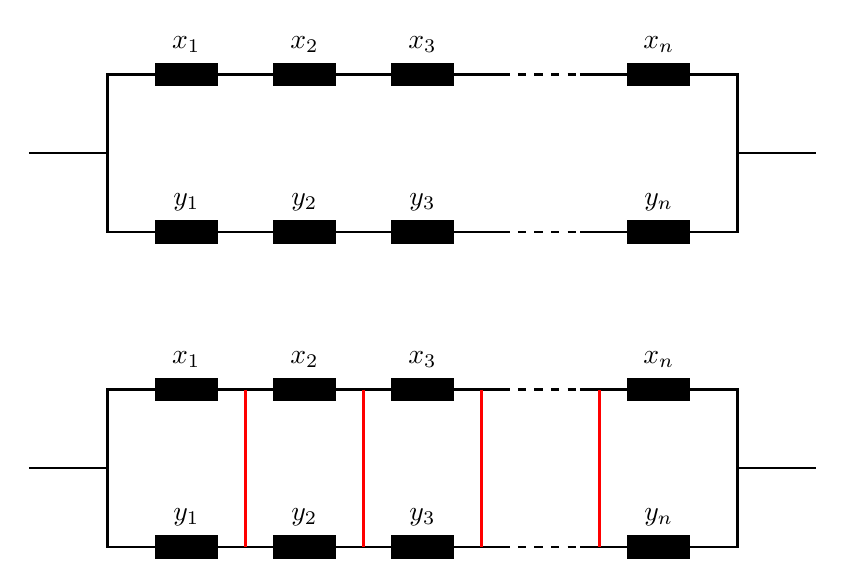
\begin{tikzpicture}[scale=1.0]
      \def\R[#1,#2,#3]{%
        \fill(#1-.4,#2)rectangle(#1+.4,#2+.3);
        \node[above] at(#1,#2+.3){#3};
      }
      \begin{scope}
        \foreach \x/\v in{0/1, 1/2, 2/3, 4/n}{
          \R[1.5*\x,0,$x_\v$]
        }
        \foreach \x/\v in{0/1, 1/2, 2/3, 4/n}{
          \R[1.5*\x,-2,$y_\v$]
        }
        \draw[thick](4,.15)--(-1,.15)--(-1,-1.85)--(4,-1.85)
                         (5,.15)--(7,.15)--(7,-1.85)--(5,-1.85)
                         (-2,-.85)--(-1,-.85)
                         (7,-.85)--(8,-.85);
        \draw[thick,dashed](4,.15)--(5,.15) (4,-1.85)--(5,-1.85);
      \end{scope}
      \begin{scope}[shift={(0,-4)}]
        \foreach \x/\v in{0/1, 1/2, 2/3, 4/n}{
          \R[1.5*\x,0,$x_\v$]
        }
        \foreach \x/\v in{0/1, 1/2, 2/3, 4/n}{
          \R[1.5*\x,-2,$y_\v$]
        }
        \draw[thick](4,.15)--(-1,.15)--(-1,-1.85)--(4,-1.85)
                         (5,.15)--(7,.15)--(7,-1.85)--(5,-1.85)
                         (-2,-.85)--(-1,-.85)
                         (7,-.85)--(8,-.85);
        \draw[thick,dashed](4,.15)--(5,.15) (4,-1.85)--(5,-1.85);
        \foreach \x in{0,1,2,3}{%
          \draw[very thick,color=red](1.5*\x+.75,.15)--(1.5*\x+.75,-1.85);
        }
      \end{scope}
    \end{tikzpicture}
  \end{center}
  考虑上下两个由若干个电阻组成的电路,上图的等效电阻为
  \begin{align*}
    \frac 1R = \frac 1{\sum x_k} + \frac 1{\sum y_k} \implies
    R = \frac{(\sum x_k)(\sum y_k)}{\sum (x_k+y_k)}
  \end{align*}
  下图的等效电阻为
  \begin{align*}
    R'=\sum \frac{x_ky_k}{x_k+y_k}
  \end{align*}
  又下图的电路中多了红色的粗导线\footnote{中间竖直的粗线。黑白印刷只能看出来粗细,可能看不出来红色。},同等条件下,参与并联的导线越多,总电阻越小,从面有$R'\le R$。
\end{proof}




